\chapter{Problem Analysis \& Solution}

Our goal is to visualize metrics suitable for arrow visualization, out of which we will restrict ourselves to the following two:

\begin{itemize}
\item Corresponding vertex distance
\item Corresponding vertex distance projected into the surface normal
\end{itemize}

Other metrics can be easily added if needed. All metrics suitable for arrow visualization can be represented by a vector. Our input to the visualization part of the process will therefore be two homologous triangle meshes with vectors saved in each vertex. Drawing these vectors directly on the screen would be counter-productive as the visualization would become too cluttered (see fig. \ref{fig:meshdiff_unclustered}). The solution is to come up with a simple abstraction for this situation and use tools available for that abstraction.

\begin{figure}[h]
\centering
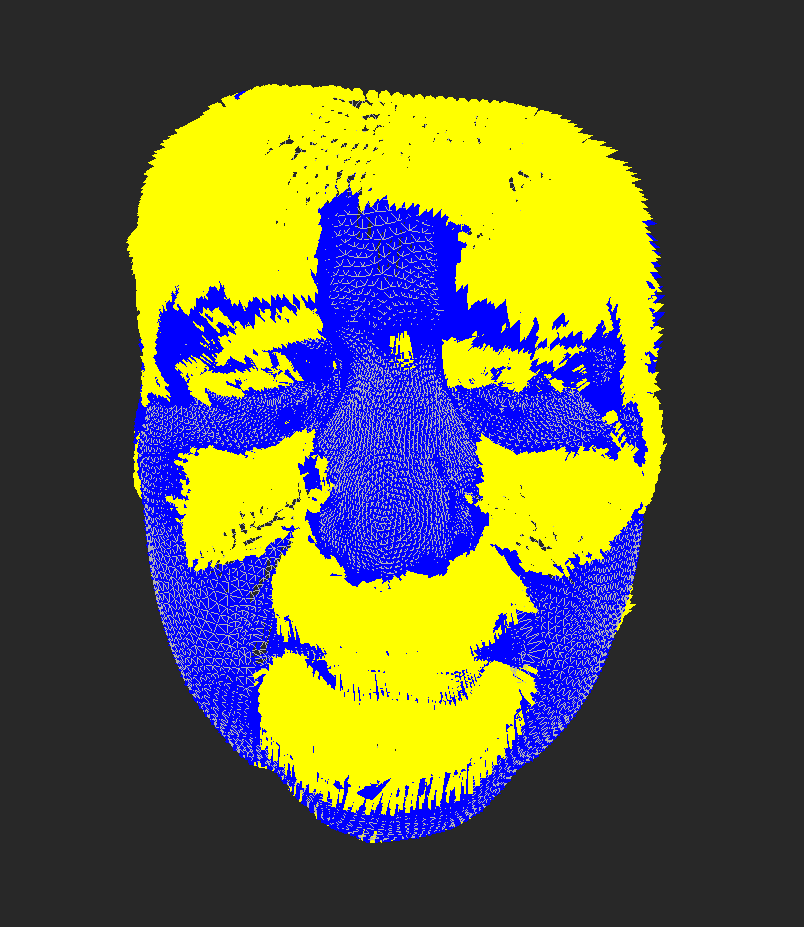
\includegraphics[width=0.5\textwidth]{./img/meshdiff-unclustered_arrows-single.png}
\caption{MeshDiff - Vertex distance visualized by unclustered arrows}
\label{fig:meshdiff_unclustered}
\end{figure}

%%-----------------------------------------------------------------------------------------
%% SECTION
%%-----------------------------------------------------------------------------------------
\section{Seeing Mesh Difference as a Vector Field}

Vectors saved in the vertices of a triangle mesh form a discrete bounded vector field. Visualization of discrete vector fields is a very active research area with applications in engineering, molecular modelling and computational fluid dynamics. There exist many scientific papers studying this topic, such as \citet{Telea99}, \citet{Garcke00}, \citet{Du04} or \citet{Peng12}.

All the above mentioned papers employ clustering techniques to reduce the number of vectors and subsequently visualize this reduced and generalized information.

%%-----------------------------------------------------------------------------------------
%% SECTION
%%-----------------------------------------------------------------------------------------
\section{Vector Field Clustering}

Clustering in general is a very subjective task (see fig. \ref{fig:clustering_subjectivity}) and there are numerous clustering techniques available. For this reason we present an overview of them to gain a better understanding of which technique might best suit our purposes and why.

\begin{figure}[h]
\centering
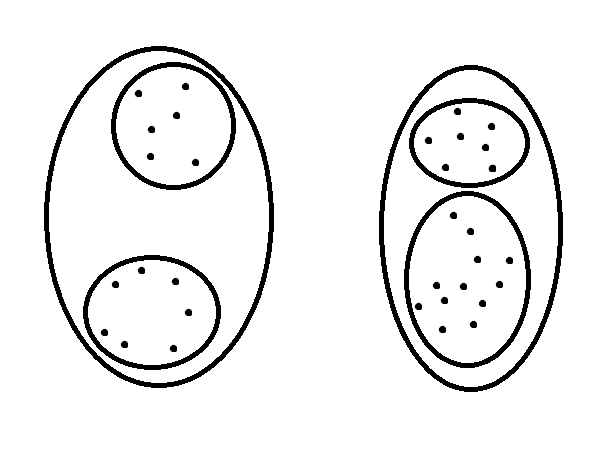
\includegraphics[width=0.6\textwidth]{./img/clustering_subjectivity.png}
\caption{The subjectivity of clustering - are there two or four clusters in the image?}
\label{fig:clustering_subjectivity}
\end{figure}

%%-----------------------------------------------------------------------------------------
\subsection{Overview of Vector Field Clustering Methods}

\citet{Telea99} use hierarchical clustering\footnotemark where neighboring clusters with the lowest clustering error are merged first. Each cluster has a representative vector and during the merge, the weighted average of the two vectors is computed and assigned to the newly formed cluster. In order to compute the clustering error, the paper introduced elliptic iso-error contours\footnotemark. This clustering method is primarily aimed at 2D rectilinear vector fields but can be also used in 3D when the error function is modified appropriately. It is possible to use up to seven parameters to configure the clustering.

\footnotetext{Hierarchical clustering, also called bottom-up clustering, starts with each data point representing an elementary cluster. In each step of the algorithm, two clustering candidates are found from the available clusters according to certain criteria and subsequently merged. Hierarchical clustering creates a binary tree, also called a dendrogram, where the each node represents a cluster and has two children from whose it was created. Arbitrary number of clusters covering the whole data set can then be obtained by taking roots of disjoint subtrees which, when combined, contain all the leaves of the dendrogram.}

\footnotetext{Clustering error in \citet{Telea99} is computed by measuring the "distance" between the representative vectors \(v, w\) of the two clusters. The elliptic iso-error contour is an ellipse which has a center on the line determined by \(v\) and intersects the apex of \(w\). All vectors \(w'\) which share the same ellipse have the same "distance" from \(v\). The shape of the ellipse and its center location can be controlled by parameters.}

\citet{Garcke00} use a continuous clustering method\footnotemark based on the physical model of \citet{CahnHilliard58} which is used to describe phase separation and coarsening in binary alloys. This model is applied to vector field data which results in a diffusion problem rather than a splitting and merging problem. Their algorithm also presumes an either 2D or 3D rectilinear grid.

\footnotetext{In continuous clustering methods, there is no notion of merging or splitting in each step of the algorithm. Instead, ``a continuous scale of successively coarser cluster sets" is created.}

\citet{Du04} use iterative clustering\footnotemark where Voronoi regions are created around the initial cluster centers and a distance function is applied to each of them. The set of cluster centers which has the lowest value of the distance function is selected as the final cluster centers set. This method works with 2D and 3D rectilinear vector fields. Clustering can be influenced by two parameters and by the distribution of the initial clusters.

\footnotetext{Iterative clustering algorithms start by assigning the data points to a given number of clusters in a random way or by using a clustering approximation. In each step, the clustering error of all clusters is computed and data points are reassigned in a way which decreases the overall clustering error.}

\citet{Peng12} use hierarchical clustering similar to \citet{Telea99}. However, the clustering is computed on a GPU by encoding a given static view of the two meshes into a rasterized image. The computation is then done for this specific image. To obtain the clustering error, a very simple formula is used:

\begin{equation} \label{eq:clustering_error}
\bm{e}(C_1,C_2) = k_d \cdot \frac{d_{C_1C_2}}{d_{max}} + k_v \cdot \frac{v_{C_1C_2}}{v_{max}} + k_\alpha \cdot \frac{\alpha_{C_1C_2}}{\alpha_{max}} + k_m \cdot \frac{m_{C_1C_2}}{m_{max}}
\end{equation}

where \(k_d + k_v + k_\alpha + k_m = 1\). The other components are the following:

\begin{itemize}
\item \(d_{C_1C_2}\) is the Euclidean distance between the positions of the representative vectors of the clusters. The maximum distance \(d_{max}\) is the length of a diagonal of the geometry's bounding box
\item \(v_{C_1C_2}\) is the difference between the lengths of the representative vectors. The maximum velocity \(v_{max}\) is the largest length in the whole data set.
\item \(\alpha_{C_1C_2}\) is angle between the representative vectors. The maximum angle \(\alpha_{max} = 180^\circ\)
\item \(m_{C_1C_2}\) is the sum of the mesh resolutions of the two clusters. \(m_{max}\) is the largest value of \(m\) in the whole data set.
\end{itemize}

The mesh resolution component also differentiates this approach from all others because it represents an approximation of the density of the mesh in a given local area. Including it in the error formula assigns higher error to dense clusters which results in a larger amount of clusters (higher precision) in dense areas of the mesh and a smaller amount of clusters (lower precision) in sparse areas of the mesh. This method is therefore aimed at non-rectilinear 3D meshes and has five parameters for user configuration (four weights and the number of clusters).
%%-----------------------------------------------------------------------------------------
\subsection{Selection Criteria for Our Clustering Method}

For our visualization purposes, we will draw inspiration from the presented clustering methods and introduce certain modifications to accommodate our needs. Here are the criteria for choosing our clustering method:

\begin{itemize}
\item Suitability for the specifics of our vector field
\item Simplicity
\item Ease of use
\end{itemize}

Methods which are suitable for our specific vector field (a triangle mesh with a vector in each vertex) will help us tailor the clustering process to achieve better results. Simple methods will allow us to quickly obtain a baseline which will help us to decide which modifications will improve the algorithm in our conditions. Lastly, the ease of configuration will make our algorithm user friendly and therefore it will increase the adoption rate.

%%-----------------------------------------------------------------------------------------
\subsection{Our Clustering Method}

We will now describe our clustering method.

\subsubsection{Clustering Algorithm}
\label{sec:analysis_clustering_algorithm}

The preference of hierarchical clustering over other mentioned clustering methods is justified by its simplicity and also the fact that a dendrogram is created during this clustering. This will allow us to quickly react to user requests for a certain number of clusters for given clustering parameters. Hierarchical clustering will also make our approach user-friendly. We will, however, introduce one optional condition to which clusters can be merged together. Since our vector fields are placed on the surface of a triangle mesh, a vector can either point "inwards" or "outwards" where the normal vector of the mesh surface is said to point "outwards". Because this might be important to the user, our clustering candidates have to not only be neighbors but also have the same orientation. The user will be able to disable this condition because the resulting dendrogram is not a tree but a forest. This may result in undesirable artifacts in the visualization because for certain cluster counts, the clustering will not cover the whole data set.

We are not going to use the GPU-based approach to clustering computations from \citet{Peng12} because it does not allow the user to view the final visualization from varying angles in real time. While one of our motivations is to have good visualizations for publishing in scientific papers, the possibility of viewing the visualizations in real time will allow the user find the ideal viewing angle more easily since it might not be known prior to the visualization process. We will store our vector field in memory and compute the clustering on the whole field in one process (similar to \citet{Telea99}).

\subsubsection{Clustering Error Function}

The error function presented in \citet{Peng12} (see Eq. \ref{eq:clustering_error}) is the only one which assumes vector fields on other than rectilinear grids. Its mesh resolution component makes it suitable to use in the clustering of vector fields on triangle meshes. The function is also simpler and more easily scalable than the elliptic iso-error contours presented in \citet{Telea99} which lead to cube root equations in 3D.

\subsubsection{Cluster Merging}

Besides clustering error computation, merging is the second crucial part of a hierarchical clustering algorithm. In the clustering of vector fields, a representative vector is usually assigned to a newly formed cluster. In our case, this shall be a weighted average of the representative vectors of the child clusters where the weight will be the geometrical area of the given cluster. Geometrical area is a better metric for cluster size than data point count because our underlying triangle mesh can have variable density.

\subsubsection{Summary}

Our clustering method will use the hierarchical algorithm and vector field representation from \citet{Telea99} with the added optional condition of merging only clusters with the same representative vector orientation relative to the mesh surface. We will use the error function \ref{eq:clustering_error} from \citet{Peng12}. Merging of two clusters will be done by computing an area-weighted average of their representative vectors and assigning the resulting vector to the newly formed cluster.
%%-----------------------------------------------------------------------------------------
%% SECTION
%%-----------------------------------------------------------------------------------------
\section{Proposed Visualizations}
\label{sec:analysis_visualizations}

Here we present the descriptions of the new visualizations which are based on the clustering process outlined above.

%%-----------------------------------------------------------------------------------------
\subsection{Arrows}
\label{sec:arrow_vis}

Once a clustering of the mesh difference vector field is obtained, representative vectors of all clusters are visualized using 3D arrows. For this purpose we have prepared a simple 3D model of an arrow which is copied to the scene at a specific position and a specific scale given by the representative vector and the cluster it belongs to.

The length of the representative vector encodes the difference metric, now averaged across the whole cluster. This length also influences the scale of the 3D arrow. Because the values of the metric can be very close to zero and because their value range is not generally very large, we have decided set a certain minimum scale and maximum scale, which is adjustable by the user, and map the metric values (vector lengths) to this interval. In general, such an approach gives a more visually pleasing and clear results, especially when the interval is chosen to be large enough.

The scale of the 3D arrows also reflects the geometrical area of the clusters. The larger the clusters are, the thicker the arrows. Areas are again mapped to a user-defined interval for clearer result. Large clusters are usually important because they represent a trend in a given area and users should be able to see them more easily and also distinguish them from less important arrows.

Lastly, and most importantly, the direction of the representative vector is directly reflected in the direction of the 3D arrow. We have therefore managed to encode three-dimensional information into our visualization.

\begin{figure}[h]
\centering
	\begin{subfigure}{0.3\textwidth}
	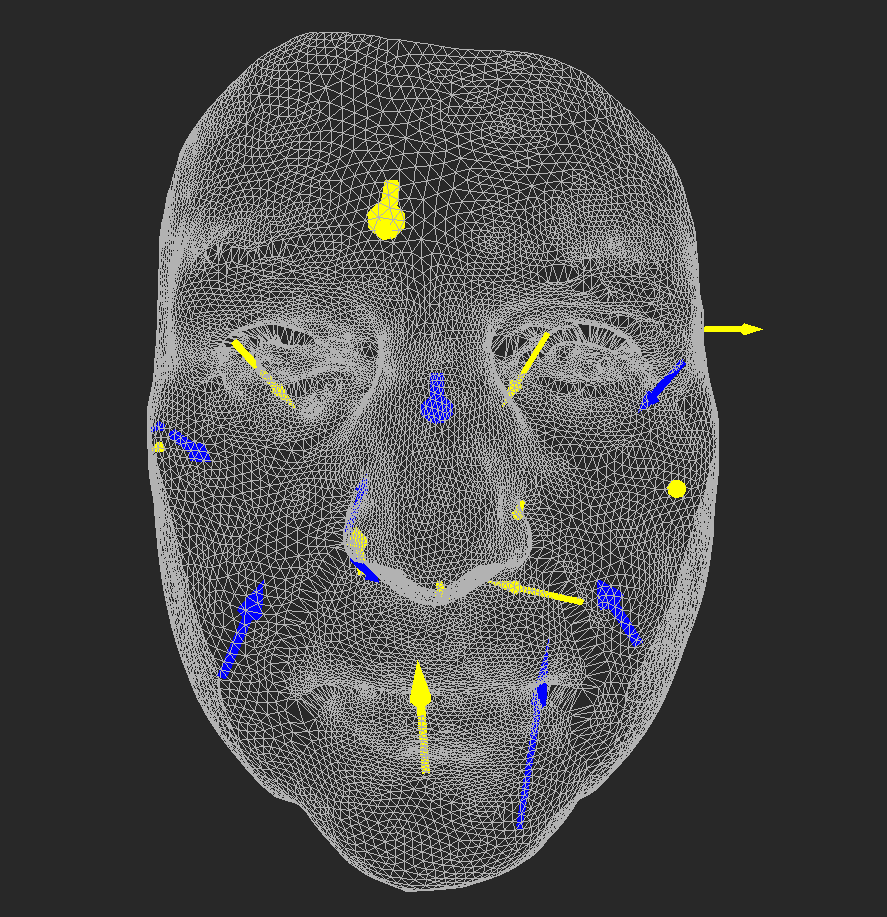
\includegraphics[width=\textwidth]{./img/meshdiff-arrows-interval0_5-5-count20-single.png}
    \caption{Smallest height \& width scale: \(0.5\); largest height \& width scale: 5; cluster count: 20}
    \label{fig:meshdiff_arrows_5-20}
	\end{subfigure}
    \qquad
    \begin{subfigure}{0.3\textwidth}
	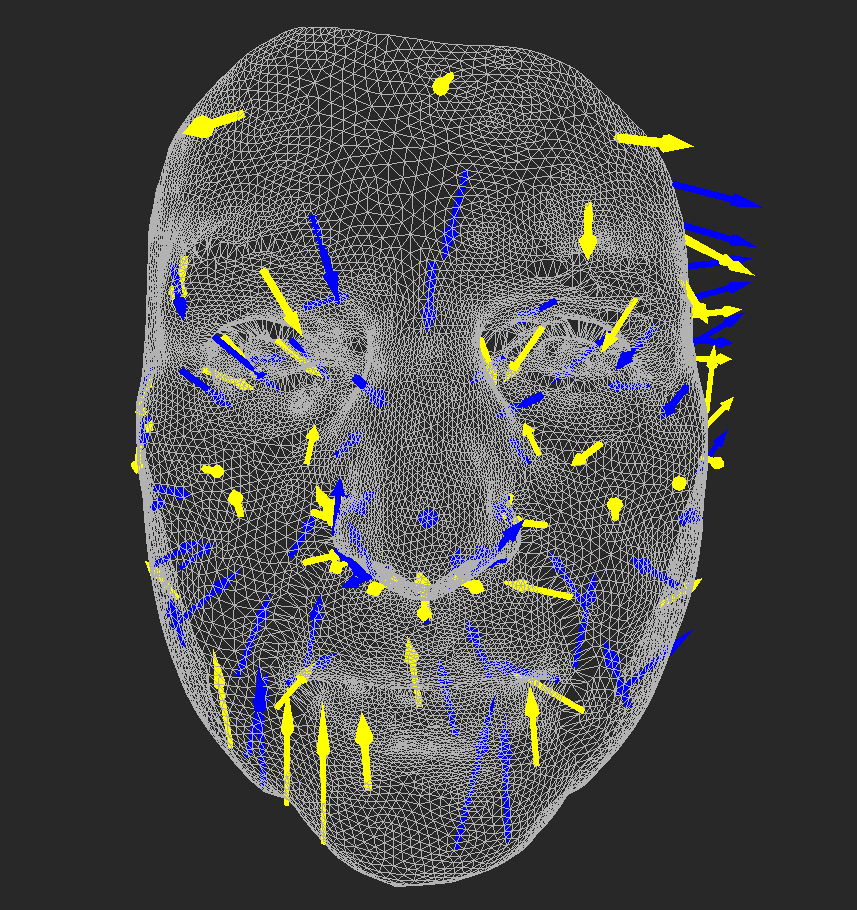
\includegraphics[width=\textwidth]{./img/meshdiff-arrows-interval0_5-5-count125-single.png}
    \caption{Smallest height \& width scale: \(0.5\); largest height \& width scale: 5; cluster count: 125}
    \label{fig:meshdiff_arrows_5-125}
	\end{subfigure}
    
    \begin{subfigure}{0.3\textwidth}
	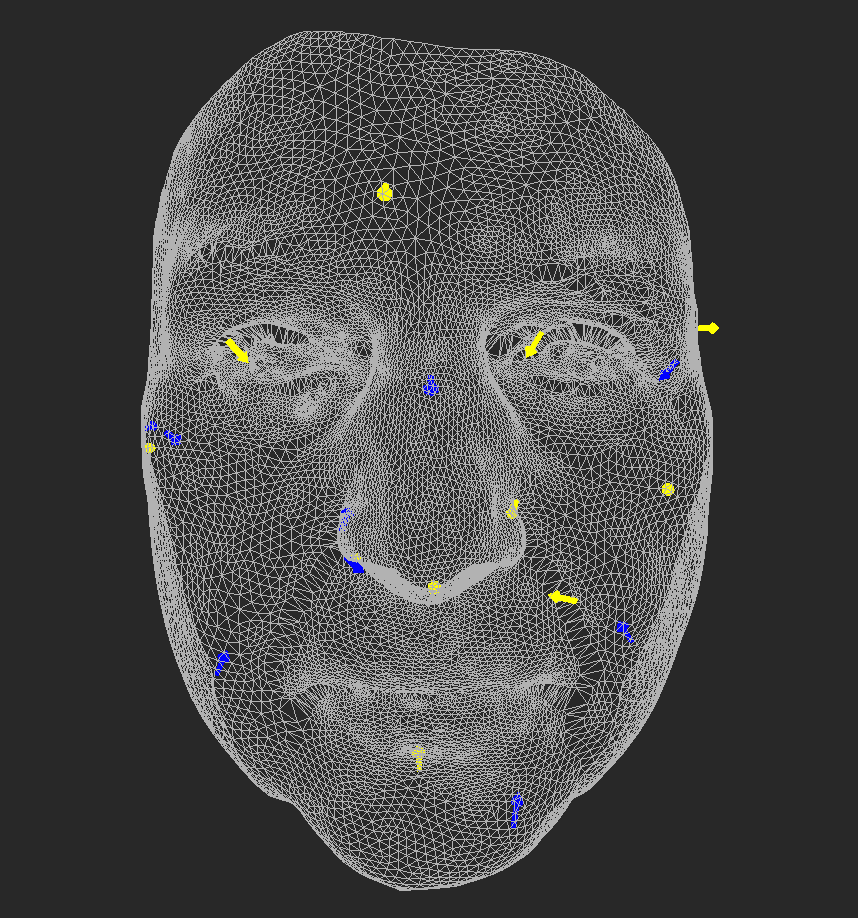
\includegraphics[width=\textwidth]{./img/meshdiff-arrows-interval0_5-1-count20-single.png}
    \caption{Smallest height \& width scale: \(0.5\); largest height \& width scale: 1; cluster count: 20}
    \label{fig:meshdiff_arrows_1-20}
	\end{subfigure}
    \qquad
    \begin{subfigure}{0.3\textwidth}
	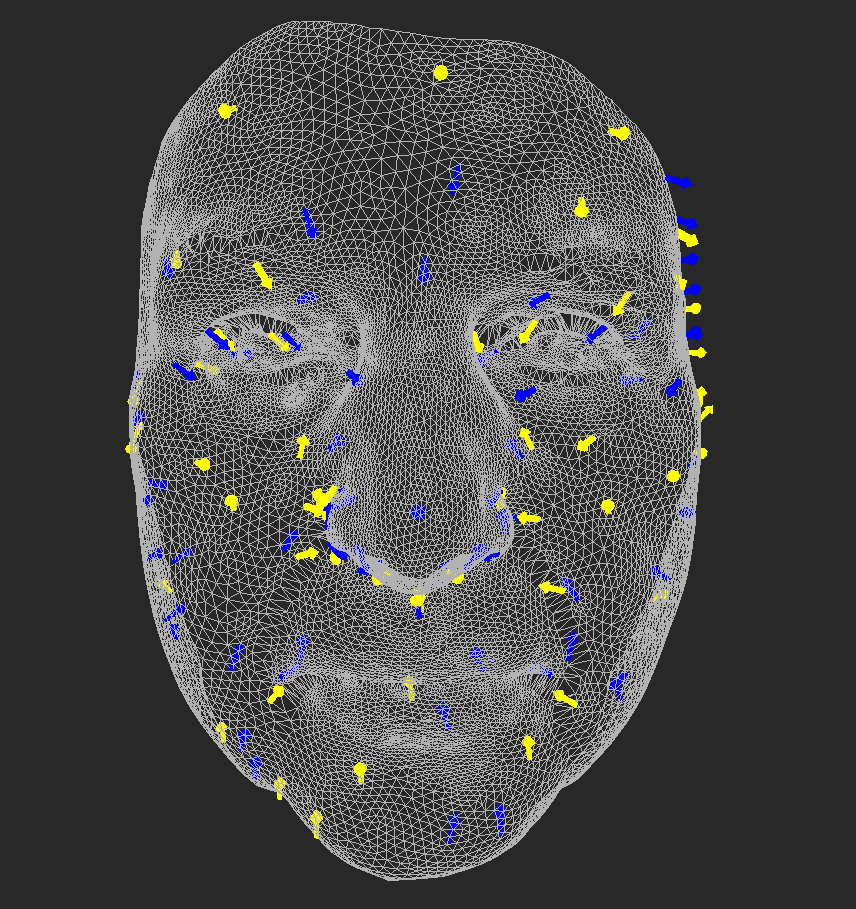
\includegraphics[width=\textwidth]{./img/meshdiff-arrows-interval0_5-1-count125-single.png}
    \caption{Smallest height \& width scale: \(0.5\); largest height \& width scale: 1; cluster count: 125}
    \label{fig:meshdiff_arrows_1-125}
	\end{subfigure}
\caption{MeshDiff - Arrow visualizations with various parameter settings}
\end{figure}

\subsubsection{Expected Performance}

Arrow visualizations combined with clustering are expected to perform well in answering questions about general trends in large parts of a mesh. They are also expected to perform considerably better than color-based visualizations when asking about the direction of the difference, which is particularly important in cases when the difference forms a very small angle with the surface of the mesh.
%%-----------------------------------------------------------------------------------------
\subsection{Cluster Color}

There are situations when the user requires clustering in order to see how larger parts of the meshes differ from one another but the richness of information offered by the arrow visualization is redundant. Also, one might simply want to see how the clustering itself behaves. For these use case we introduce two color visualizations of clusters - random and metric-based.

Both of these visualizations need to be aware of which mesh vertices belong to a given cluster. Then either a random color is assigned to all vertices in a given cluster or a color based on the length of the representative vector of the cluster is assigned. The former case is basically the original color visualization of a metric, only applied on clusters.

We propose two modes of assigning the color to the vertices based on metrics, the relative mode and the absolute mode. In both modes, a distinct user-defined color hue is assigned to clusters whose representative vectors point "inwards" and "outwards". What differs is the shade assigned to clusters of specific metric value.

In the relative mode, the highest and lowest metric values are taken first. The lowest value receives a black color and the highest value receives the brightest user-defined color. All other values are mapped to this interval and receive a color which is a proportional mixture of the user-defined color and black.

In the absolute mode, black color is assigned to cluster of zero metric value and the brightest color is assigned to clusters of metric value higher or equal than a user-defined value. This allows the user to compare across several visualizations and determine the absolute value of the difference metric more easily.

\begin{figure}[h]
\centering
	\begin{subfigure}{0.3\textwidth}
	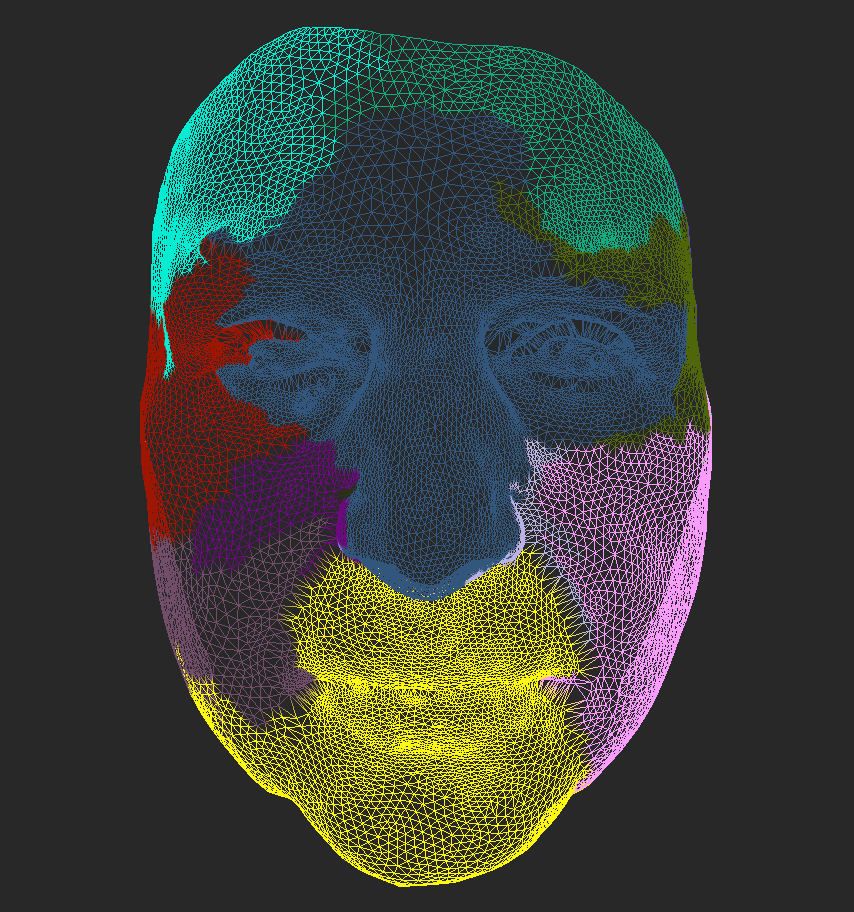
\includegraphics[width=\textwidth]{./img/meshdiff-clustercolor-random.PNG}
    \caption{Random cluster colors}
    \label{fig:meshdiff_clustercolor_random}
	\end{subfigure}
    \qquad
    \begin{subfigure}{0.3\textwidth}
	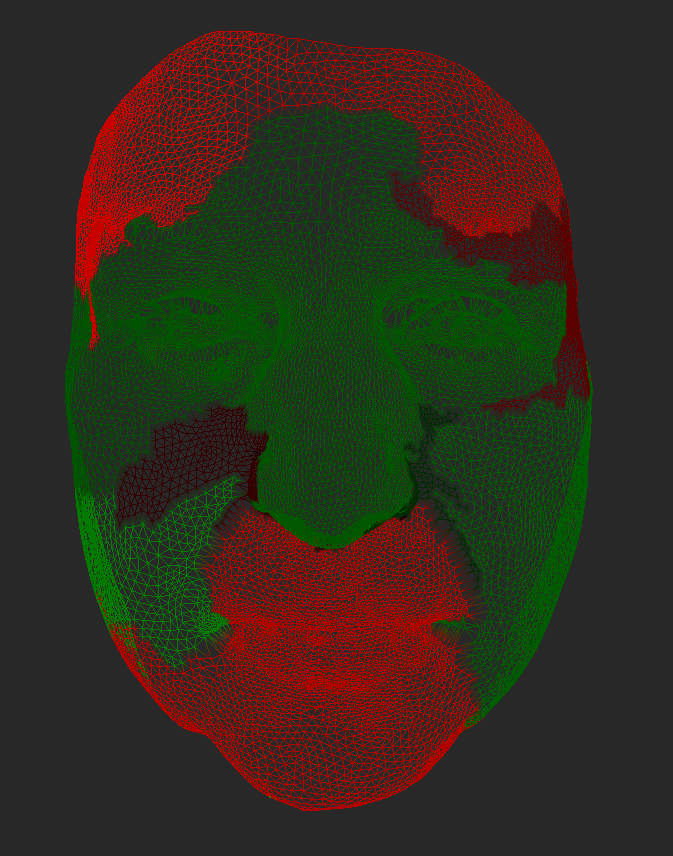
\includegraphics[width=\textwidth]{./img/meshdiff-clustercolor-metric.PNG}
    \caption{Metric-based cluster colors}
    \label{fig:meshdiff_clustercolor_metric}
	\end{subfigure}
    
\caption{MeshDiff - Cluster color visualizations}
\end{figure}

\subsubsection{Expected Performance}

Random cluster color is expected to be used for the purpose of configuring the clustering parameters as the size and the location of the clusters is clearly visible in this case.

Metric-based cluster color is expected to perform well in cases when we have found the most important differences using a more sophisticated visualization and want to present those using a visualization which is as clear as possible.
%%-----------------------------------------------------------------------------------------
\subsection{Thresholding}

For all types of metric-based visualizations, including the original color-based ones, we present thresholding. Each vertex or cluster which does not have a sufficiently high metric value assigned to it is excluded from the visualization. This method therefore works as a high-pass filter on the visualization.

\begin{figure}[h]
\centering
	\begin{subfigure}{0.3\textwidth}
	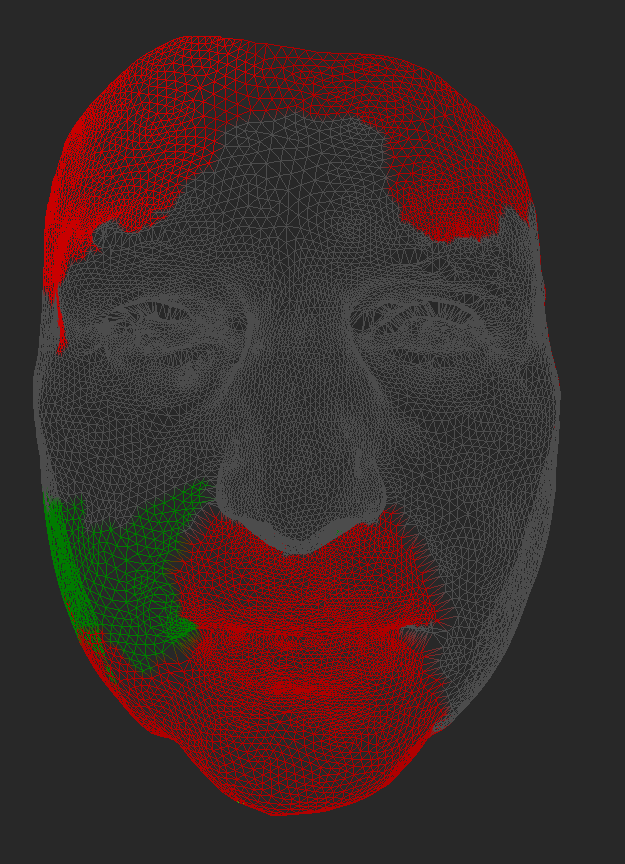
\includegraphics[width=\textwidth]{./img/meshdiff-thresholding-clustercolor-length3.PNG}
    \caption{Clusters with distance less than 3 grayed out}
    \label{fig:meshdiff_thresholding_clustercolor}
	\end{subfigure}
    \qquad
    \begin{subfigure}{0.3\textwidth}
	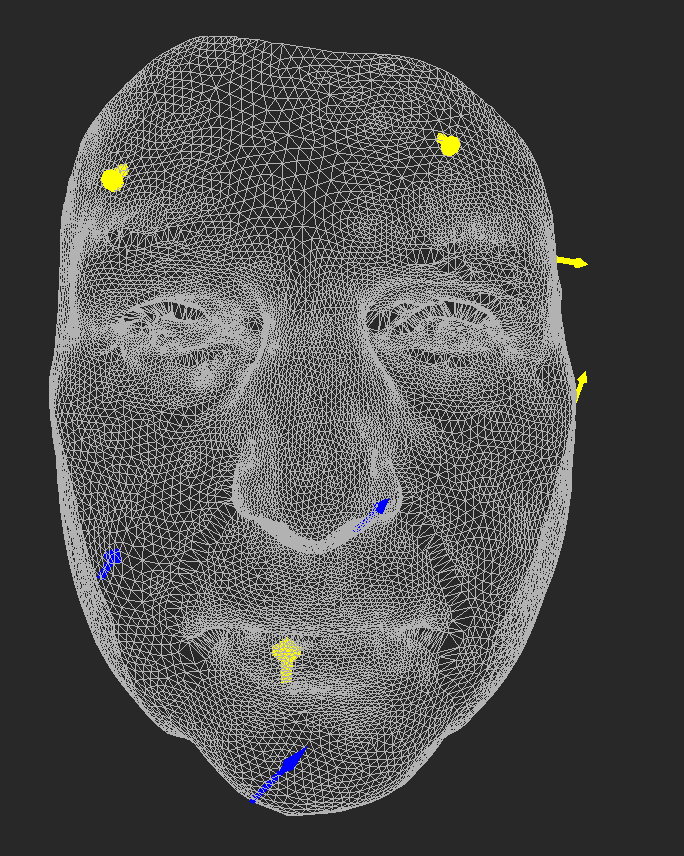
\includegraphics[width=\textwidth]{./img/meshdiff-thresholding-arrows-length3.PNG}
    \caption{Arrows for cluster with distance less than 3 excluded}
    \label{fig:meshdiff_thresholding_arrows}
	\end{subfigure}
    
\caption{MeshDiff - Thresholded visualizations}
\end{figure}

\subsubsection{Expected Performance}

Thresholding is expected to enhance the effect of metric-based cluster color in that it is expected to perform very well when segmenting and emphasizing a previously discovered difference which is of importance to the user. It is also expected to help answer questions about the largest differences in the mesh.
%%-----------------------------------------------------------------------------------------
\subsection{Combined Visualizations}

The last visualization type presented in this thesis is the combination of color and arrow visualizations.

\begin{figure}[h]
\centering
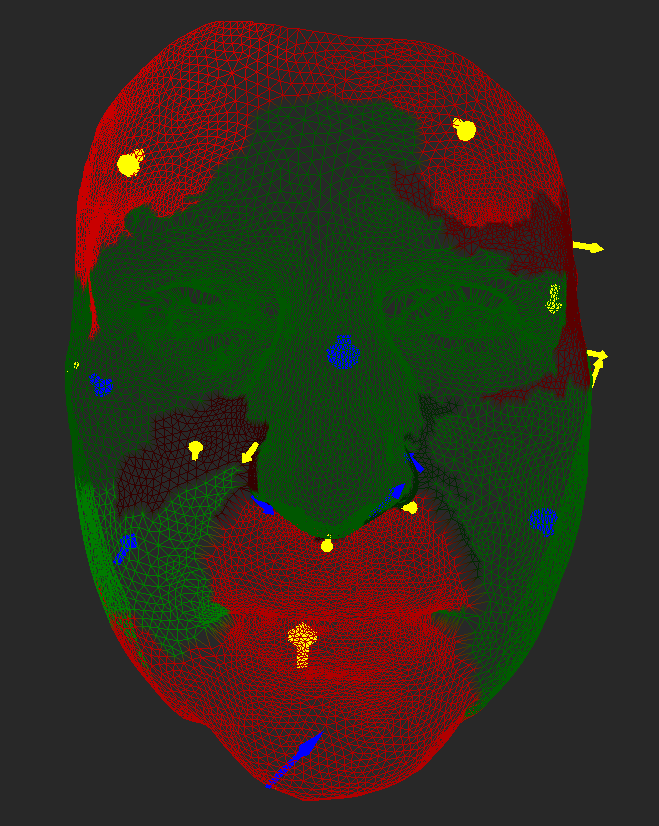
\includegraphics[width=0.5\textwidth]{./img/meshdiff-combination.PNG}
\caption{MeshDiff - Combined visualization}
\label{fig:meshdiff_combination}
\end{figure}

\subsubsection{Expected Performance}

Combined visualizations complement each other in areas when only one visualization is not sufficiently clear. Color visualizations are expected to highlight the dimension of the metric we are interested in the most, for example vertex distance magnitude, while arrow visualization are expected to carry the other dimensions like direction and cluster size. This method is expected to bring a balance between clarity and information richness.
%%-----------------------------------------------------------------------------------------
%% SECTION
%%-----------------------------------------------------------------------------------------
\section{Effect of Clustering Parameters on the Visualizations}
\label{sec:parameter_effect}

The function used for computing the clustering error (see eq. \ref{eq:clustering_error}) has four parameters:

\begin{itemize}
\item Direction weight
\item Position weight
\item Magnitude weight
\item Resolution weight
\end{itemize}

A specific configuration of these parameters can influence the outcome of the clustering process considerably. Setting the value of one of them higher than the others will cause the proportion of the corresponding part of the clustering error be higher than the others. This will make that part of the error more significant and cause cluster pair with low values in this area merge much easier than all the other cluster pairs.

%%-----------------------------------------------------------------------------------------
\subsection{Direction Weight}

High direction weight causes clusters whose representative vectors have similar directions merge easily regardless of their difference in position, magnitude and resolution. This results in uneven cluster sizes. It forms many small clusters in areas of high surface curvature and large clusters in flat areas. Therefore, it mostly captures the high-curvature changes of shape.
%%-----------------------------------------------------------------------------------------
\subsection{Position Weight}

Setting the position weight higher than others results in clusters of even size where each of them represents the overall difference in a certain area regardless of the variety of directions and magnitudes in that area.
%%-----------------------------------------------------------------------------------------
\subsection{Magnitude Weight}

Magnitude weight can play a significant role when using the metric-based cluster color visualization because its high value will highlight iso-magnitude contours. Such an approach can be useful when grouping and segmenting areas with a certain absolute value of the difference metric.
%%-----------------------------------------------------------------------------------------
\subsection{Resolution Weight}

High resolution weight prefers clustering in sparse areas of the mesh and will therefore increase the precision of the visualization in very dense areas. This effect partially complement direction weight because high-curvature areas of triangle meshes are usually more dense for the high-curvature to be captured well.

\begin{figure}[h]
\centering
	\begin{subfigure}{0.3\textwidth}
	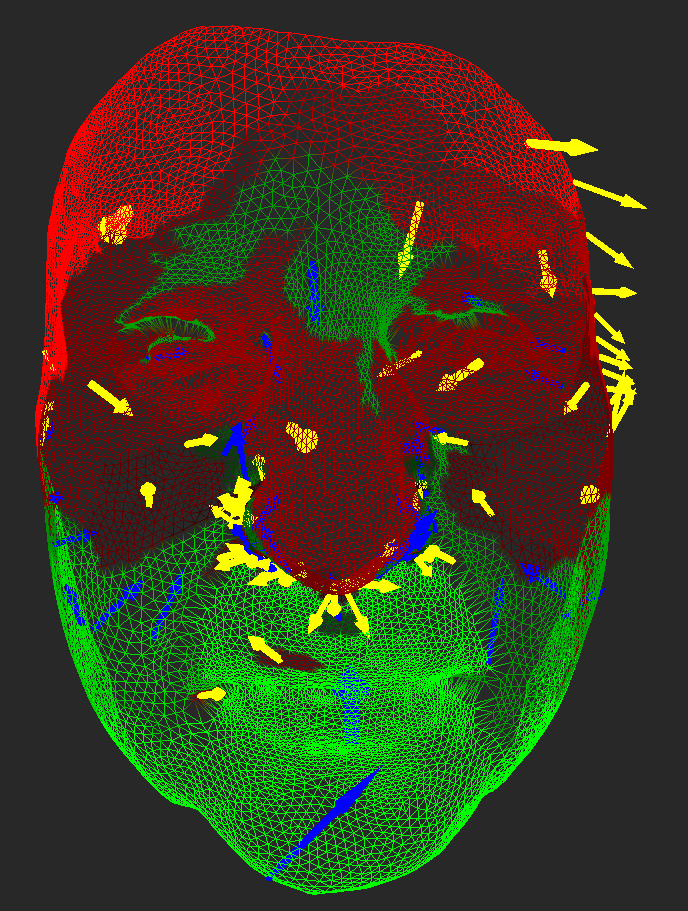
\includegraphics[width=\textwidth]{./img/meshdiff-high_direction.PNG}
	\caption{High direction weight}
	\label{fig:meshdiff_high_direction}
	\end{subfigure}
    \qquad
    \begin{subfigure}{0.3\textwidth}
	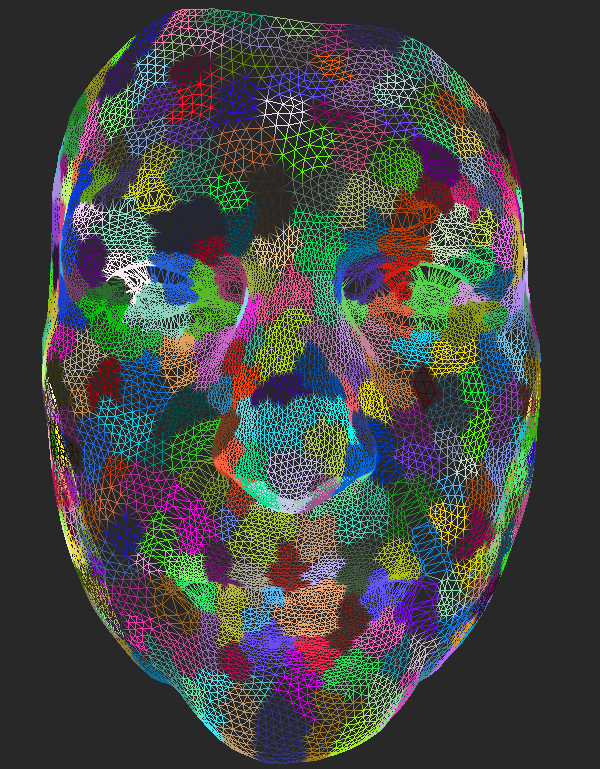
\includegraphics[width=\textwidth]{./img/meshdiff-high_position.PNG}
	\caption{High position weight}
	\label{fig:meshdiff_high_position}
	\end{subfigure}
    
    \begin{subfigure}{0.3\textwidth}
	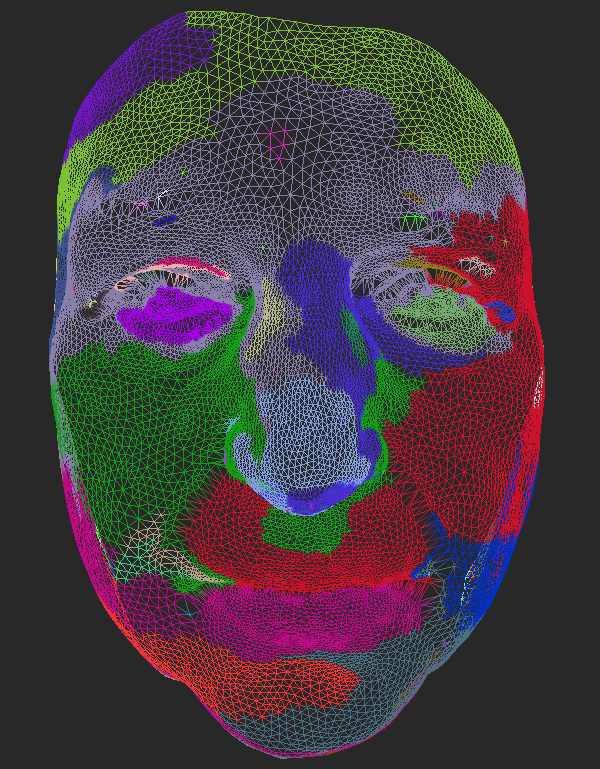
\includegraphics[width=\textwidth]{./img/meshdiff-high_magnitude.PNG}
	\caption{High magnitude weight}
	\label{fig:meshdiff_high_magnitude}
	\end{subfigure}
    \qquad
    \begin{subfigure}{0.3\textwidth}
	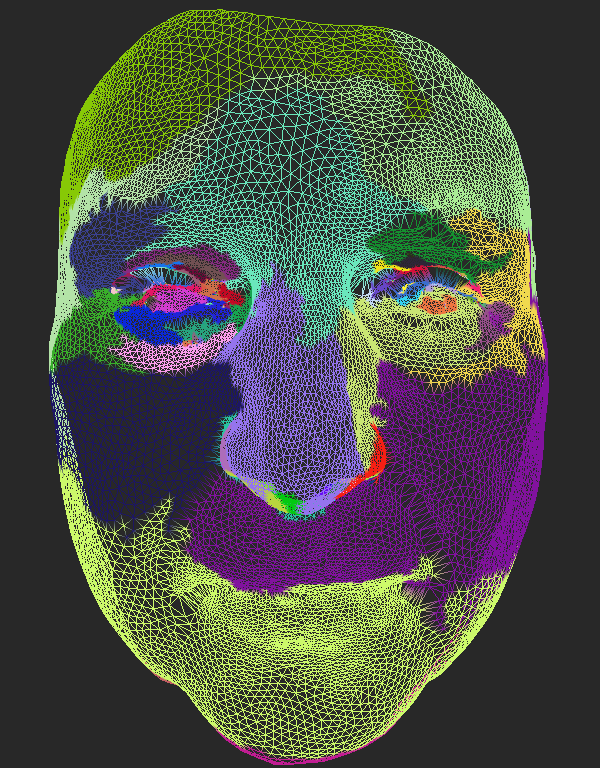
\includegraphics[width=\textwidth]{./img/meshdiff-high_resolution.PNG}
	\caption{High resolution weight}
	\label{fig:meshdiff_high_resolution}
	\end{subfigure}
\caption{MeshDiff - Various clustering parameter settings}
\end{figure}

%%-----------------------------------------------------------------------------------------
%% SECTION
%%-----------------------------------------------------------------------------------------
\section{MeshDiff Application}

Our intention is to create an application which will allow us to demonstrate the proposed visualizations, conduct a user study and also provide basic features for users who wish to experiment with visualizations of their own data and potentially publish the visualizations without any extra implementation work.

Just like in MeshLab or Morphome3cs, in Mesh Diff, the core functionality is the ability to load and store triangle meshes and to view them interactively using the mouse cursor. We will build features specific for mesh difference visualizations on top of this basis.

%%-----------------------------------------------------------------------------------------
\subsection{Features}
\label{sec:meshdiff_features}

We will now briefly mention the features of Mesh Diff related to mesh difference visualization and the rationale behind them.

\subsubsection{Two Viewing Panels}

Mesh contains two viewing panels, therefore two triangle meshes can be loaded next to each other at the same time. This makes the difference visualizations much more powerful and clear because the user can see what the difference is related to.

We have also added an option for the user to control the viewing angle and zoom of both meshes at the same time. Thanks to this feature, it is easier to find the same area of interest in both meshes and examine it further.

\begin{figure}[h]
\centering
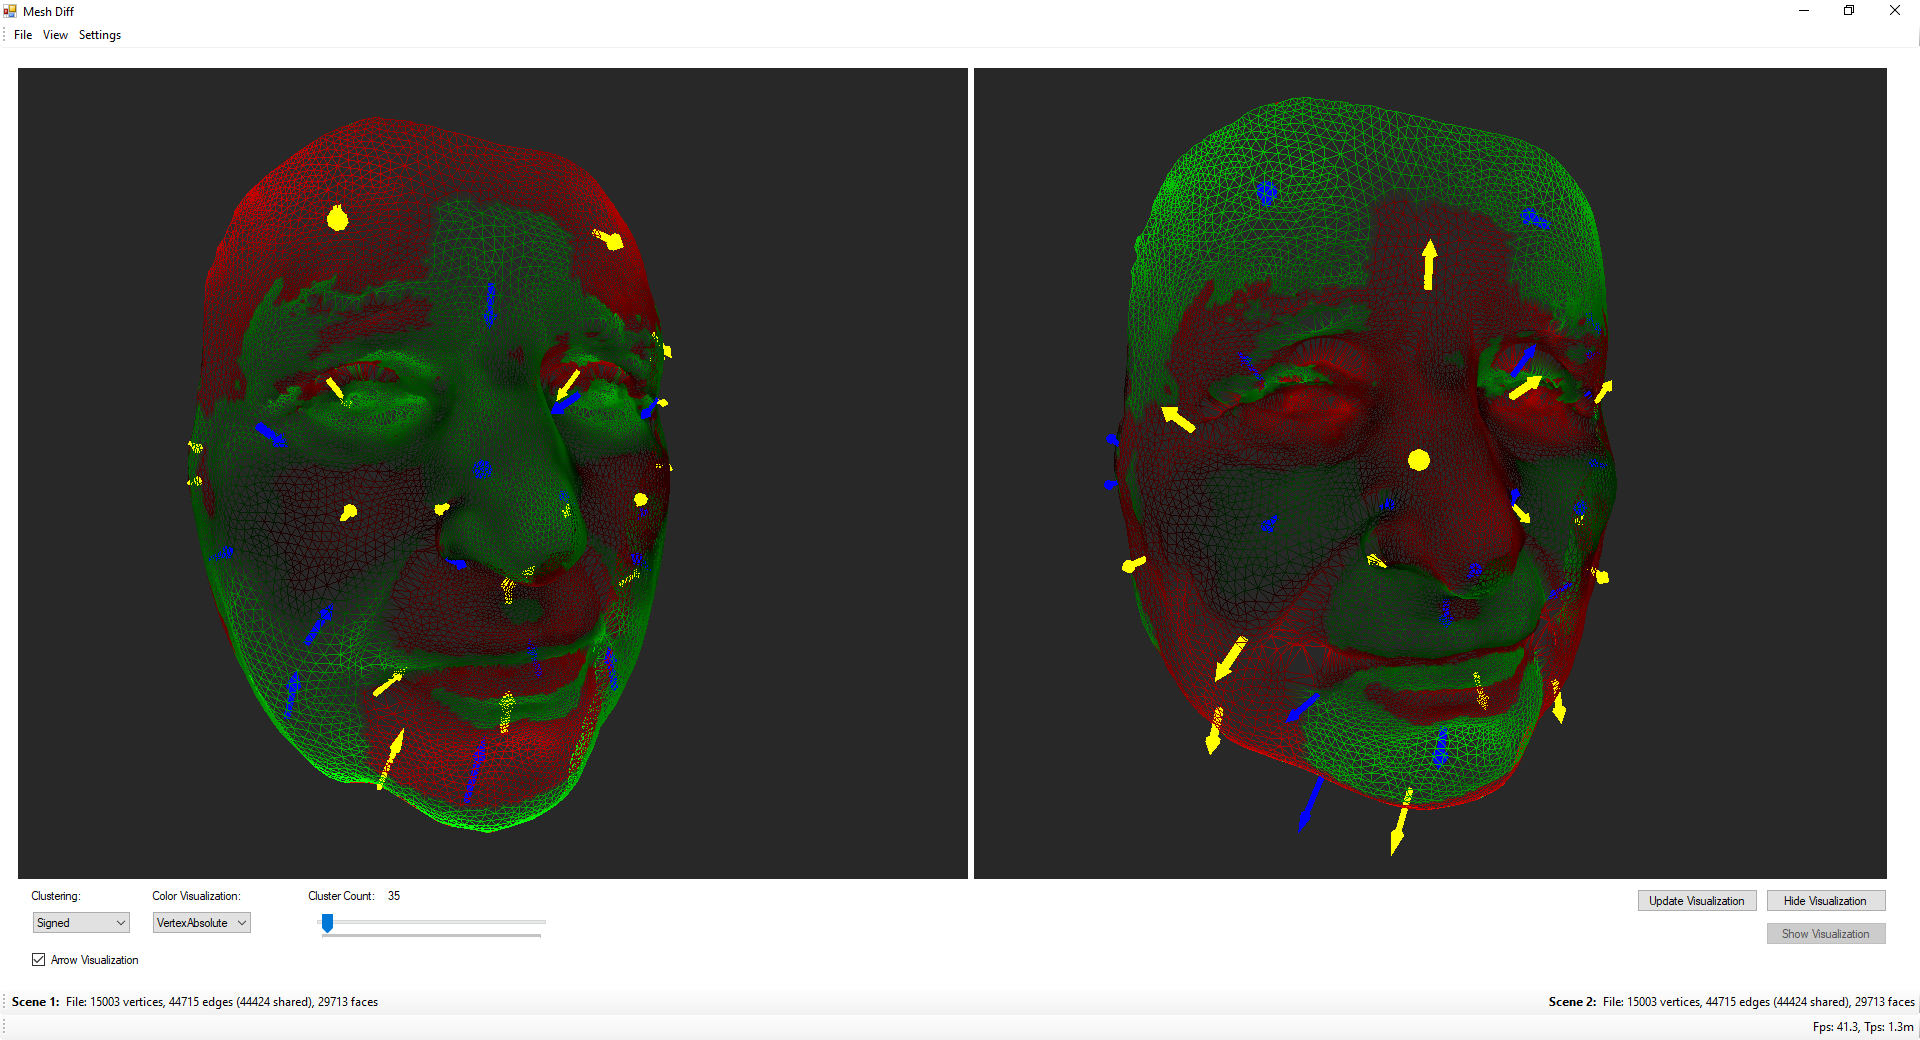
\includegraphics[width=\textwidth]{./img/meshdiff.PNG}
\caption{MeshDiff - Application view}
\label{fig:meshdiff}
\end{figure}

\subsubsection{Visualization Configuration and Generation}

The difference metric to be used, all clustering parameters (see section \ref{sec:parameter_effect}), visualization parameters (arrow size and color, thresholding, etc.) and the chosen visualization type form a configuration of the visualization process. This configuration can be fully customized in the user interface where the user can also generate a visualization and then toggle its visibility. Such a feature is vital for the full demonstration of the proposed methods.

\subsubsection{Visualization Store and Load}

Mesh Diff supports loading and storing of visualizations in the standard \verb+.ply+ format. The format was chosen because it is able to store color in vertices which makes it easier to work with than for example \verb+.obj+ where additional textures would have to be used for storing color. 

Arrows (\ref{sec:arrow_vis}) can be stored to separate \verb+.ply+ files and also loaded from them which increases the variability of the application.

\subsubsection{Configuration Store and Load}

Visualization configuration including the viewing angle and zoom value can also be stored to a file and subsequently loaded. Replication, demonstration and publication of specific visualizations is much easier with this feature.
%%-----------------------------------------------------------------------------------------
\subsection{Platform}

Mesh Diff is written in C\#, its user interface is created in WinForms and rendering is handled by the OpenTK library which provides an interface to OpenGL in C\#. The reason for this choice is that we have available code written by Josef Pelikán which supports exactly those features that were mentioned at the beginning of this section and is easily extensible to support the extra features we have outlined above. Because MeshDiff is mainly of experimental nature and is only meant for the demonstration of visualization algorithms, the only targeted operating system is Windows.